\documentclass[12pt]{article}
\usepackage[T1]{fontenc}
\usepackage{listings}
\usepackage{tikz}
\usepackage{booktabs}
\usepackage{tabularx}
\usepackage{array}
\usepackage{titlesec}
\usepackage[a4paper, margin=1in]{geometry}
\usepackage[hidelinks]{hyperref}
\usepackage{placeins}
\usepackage{float}
\usepackage{color}
\usepackage{rotating}
\definecolor{mygreen}{rgb}{0,0.6,0}
\definecolor{mygray}{rgb}{0.5,0.5,0.5}
\definecolor{mymauve}{rgb}{0.58,0,0.82}
\hypersetup{
	colorlinks,
	citecolor=black,
	filecolor=black,
	linkcolor=black,
	urlcolor=black
}
\setcounter{tocdepth}{4}
\setcounter{secnumdepth}{4}
\begin{document}
	\title{\huge Rescue on wheels project documentation}
	\author{\\Team 2\\ \\Damian de Hoog 500780277\\ Yoshio Schermer 500760587\\Mustafa Y\"{u}cesan 500769574\\ Mohamed El Hadiyen 500777214}
	\maketitle
	\newpage
	\tableofcontents
	\newpage
	\section{Introduction}
	This document contains all the information regarding "Metabot" our rescue on wheels project. This document will describe the design phase, working phase and post-launch phase consisting of:
	\begin{itemize}
		\item An analysis of the requirements for the project from the perspective of an user.
		\item A design model which explains in great detail how the system is built.
		\item Documentation containing important code segments with comments and explanations as well guidance for installation, operation and maintenance.
	\end{itemize} 
	Metabot is a Raspberry Pi powered mobile robot designed to assist in rescue operations. The robot will be able to navigate difficult to traverse environments and explore areas as a sort of reconnaissance unit.\\
	Metabot is equipped with a camera which will broadcast to a mobile device on which the user can control the robot as well as see said camera feed. The camera has a facial recognition functionality to assist in spotting survivors.\\
	Whilst navigating the operating environment Metabot will map the area and ping locations on the map when survivors are found.\\ 
	\\Metabot will be able to explore and create a map of the area with the locations of survivors. This way, having seen the environment and knowing the locations of the survivors,  the rescue team will be able to conduct a swift and efficient rescue operation.\\
	\\The following chapters will describe the robot in more details as well as it's design. We will begin with the analysis of the requirements for the Metabot. 
	\newpage
	\section{Analysis}
	The analysis consists of the following parts:
	\begin{itemize}
		\item Epic
		\item User stories
		\item Use-cases
		\item Use-case diagram
		\item Domain model\\
	\end{itemize}	
	The analysis answers the question of "How, in detail, is the product designed?"\\
	\\The formulation of the requirements was performed based on user stories. These user stories were created based on an epic. An agile epic is a body of work that can be broken down into specific tasks (called ''stories,'' or ''user stories'') based on the needs/requests of customers or end users\footnote{https://www.atlassian.com/agile/project-management/epics}.\\
	\\After having created said requirements we will formulate the Use-case diagram(s) and the Domain model(s). These will visualize the user interaction with our system and our Metabot.
	\subsubsection{Terms and definitions}
	Below you'll find the terms and definitions used throughout this document.
	\begin{table}[H]
		\centering
		\begin{tabularx}{\linewidth}{|X|X|}
			\hline
			\textbf{Terms} &\textbf{Definitions}\\
			\hline
			Rover &Remotely-controllable RC-car with sensors attached to it.\\
			\hline
			App &The mobile app through which the rover can be remotely-controlled.\\
			\hline
			Rover operator &An individual who operates the rover.\\
			\hline
			Web interface &The web interface through which the rover can be remotely-controlled. \\
			\hline 
			Livestream &A livestream of the camera feed that is attached to the rover.\\
			\hline
		\end{tabularx}
		\caption{Terms and definitions for this document.}
		\label{table:termsDefinition}   
	\end{table}
	\newpage
	\subsection{Epic}
	 A building has collapsed trapping the people inside. Some managed to get out in time but others weren't so lucky. Upon arrival at the scene our actor assesses the situation. The building is unstable and the trapped survivors need to be rescued as quickly as possible.\\
	 \\Normally a rescue crew would be assembled and they would slowly make their way through the rubble to search for people. This is a dangerous and time-consuming task. The crew has no idea whether or not there is a way to get to the survivors. Removing rubble could make the building collapse even further. These people need to be found and removed from the ruins before this happens.\\
	 \\Luckily our actor has just the tool for this job. The Metabot, a small remote controlled robot that can do the scouting for our actor. Our actor takes out his phone and boots up the app. Here, our actor can control the robot.\\
	 \\Our actor sends the robot into the ruins, slowly making it's way deeper and deeper into the building. Whilst moving, the robot sends out signals to its surroundings to map the area and to avoid collision with objects. Meanwhile, our actor can see what the robot is seeing through the live camera feed. Our actor uses this feed to try and find survivors while also looking around for possible routes to take with the rescue crew.\\
	 \\Once our actor has found a survivor, the robot's facial recognition software will help our actor detect the survivor. After this detection, the robot will ping the location of the survivor on the map so that our actor knows where in relation to the rest of the building the survivors are. After pinging the location, the robot will give a visual light signal to the survivors to let them know they have been found and will soon be rescued.\\
	 \\After mapping the area and locating the survivors our actor can create a rescue plan and execute it. Having performed reconnaissance safely and quickly with the Metabot, our rescue crew can now swiftly save the survivors. 
	 \newpage
	\subsection{User stories}
	 From this epic story we could formulate user stories, this resulted in the following table:
	 \begin{table}[H]
	 	\centering
	 	\begin{tabularx}{\linewidth}{|X|X|X|X|}
	 		\hline
	 		\textbf{M: As operator I want to be able to recognize a survivor's face, so I can get information about this survivor.}                                               &\textbf{M: As operator I want to visually explore the environment from a distance, so I can be better prepared for the rescue operation.}       &\textbf{S: As operator I want to know the locations of the survivors in relation to the environment, so that I know where I can find the survivors.}
	 		                                                        &\textbf{S: As a survivor I want to know if I have been found, so I can be rescued.}
	 		                                                                                    \tabularnewline \hline
	 		As operator I want a mobile robot to recognize a survivor's face, so I can get information about this survivor                                              &As operator I want the mobile robot to show me the environment on a screen at a distance so that I can plan the rescue operation accordingly.                                          &As operator I want a mobile robot to tell a mobile app where the survivor is in relation to the environment, so that I know where I can find the survivors.                                            &As survivor I want the mobile robot to give me a sign, so I know I have been found.
	 		\tabularnewline \hline
	 		As operator I want a mobile app to get the information that corresponds to the survivor's face, so I know who the survivor is.                                                   &As operator I want the mobile robot to stream the camera feed to a mobile device so I can get real time information from the environment.   &As operator I want a mobile app to display where the survivors are in relation to the environment, so that I know where I can find the survivors. &   \tabularnewline \hline
	 	                                               &As operator I want to control the mobile robot from a distance to plan the rescue operation accordingly.  & &
            \tabularnewline \hline
	 	\end{tabularx}
	 	\caption{User stories formed in accordance with the epic story.}
	 	\label{table:userStories}   
	 \end{table}
 	
 	\subsection{Use-cases}
	 	\begin{table}[H]
	 	\centering
		 	\begin{tabularx}{\linewidth}{|X|X|}
		 		\hline
		 		\textbf{Use Case ID:} &1\\
		 		\hline
		 		\textbf{Use Case Name:} &Connect with rover\\
		 		\hline
		 		\textbf{Primary Actor:} &Rover operator\\
		 		\hline
		 		\textbf{Secondary Actor:} &Rover\\
		 		\hline
		 		\textbf{Pre-conditions:} &\begin{enumerate}
		 			\item Rover operator has mobile app or address of web interface.
		 			\item Rover is nearby.
		 		\end{enumerate}\\
		 		\hline
		 		\textbf{Success Guarantee:} &Rover operator successfully connected the mobile app/web interface to the rover. \\
		 		\hline 
		 		\textbf{Main Success Scenario:} &\begin{enumerate}
		 			\item Rover operator opens app or goes to the web interface.
		 			\item Rover operator searches for rover to connect to within the app.
		 			\item Rover operator selects rover to connect to.
		 			\item Rover operator confirms to connect to the selected rover.
		 			\item Rover operator successfully connected the app/web interface to the rover.
		 		\end{enumerate}\\
		 		\hline
		 		\textbf{Exceptions} &\begin{itemize}
		 			\item Rover operator already has established a connection between the app/web interface and the rover.
		 			\item Rover operator cannot connect app/web interface to the rover, because the rover is already connected with the same app/web interface from another rover operator.
		 			
		 		\end{itemize}\\
		 		\hline
		 		\textbf{Special Requirements} &- \\
		 		\hline
		 	\end{tabularx}
		 	\caption{Use-case 1}
		 	\label{table:Use-case1}   
	 	\end{table}
	 	\begin{table}[H]
	 		\centering
	 		\begin{tabularx}{\linewidth}{|X|X|}
	 			\hline
	 			\textbf{Use Case ID:} &2\\
	 			\hline
	 			\textbf{Use Case Name:} &Look for survivors on flat surfaces\\
	 			\hline
	 			\textbf{Primary Actor:} &Rover operator\\
	 			\hline
	 			\textbf{Secondary Actor:} &Rover\\
	 			\hline
	 			\textbf{Pre-conditions:} &\begin{enumerate}
	 				\item Rover operator has established a connection between the app /web interface and the rover.
	 				\item Rover operator sees what the rover sees.
	 				\item Rover operator has controller.
	 			\end{enumerate}\\
	 			\hline
	 			\textbf{Success Guarantee:} &
	 			Rover operator uses the rover to look for survivors on flat surfaces, that is, drives around. \\
	 			\hline 
	 			\textbf{Main Success Scenario:} &\begin{enumerate}
	 				\item Rover operator uses controller to drive either forward, backward, left, or right.
	 				\item Rover operator uses the live stream to look for any survivors.
	 			\end{enumerate}\\
	 			\hline
	 			\textbf{Exceptions} &-\\
	 			\hline
	 			\textbf{Special Requirements} &-\\
	 			\hline
	 		\end{tabularx}
	 		\caption{Use-case 2}
	 		\label{table:Use-case2}   
	 	\end{table}
	 	\begin{table}[H]
	 		\centering
	 		\begin{tabularx}{\linewidth}{|X|X|}
	 			\hline
	 			\textbf{Use Case ID:} &3\\
	 			\hline
	 			\textbf{Use Case Name:} &Know who a survivor is and where they are\\
	 			\hline
	 			\textbf{Primary Actor:} &Rover operator\\
	 			\hline
	 			\textbf{Secondary Actor:} &Rover\\
	 			\hline
	 			\textbf{Pre-conditions:} &\begin{enumerate}
	 				\item Rover operator has established a connection between the app/web interface and the rover.
	 				\item Rover operator sees what the rover sees.
	 				\item Rover operator has controller.
	 			\end{enumerate}\\
	 			\hline
	 			\textbf{Success Guarantee:} &Rover operator drives around with the rover. Through the livestream the rover operator can see who the survivor is and where they are to be seen. \\
	 			\hline 
	 			\textbf{Main Success Scenario:} &\begin{enumerate}
	 				\item Rover operator uses controller to drive either forward, backward, left, or right.
	 				\item Rover operator uses the live stream to look for any survivors.
	 				\item A survivor’s face is visible through the livestream.
	 				\item Through the livestream the rover operator can tell who the survivor is and where the face of the survivor is.
	 			\end{enumerate}\\
	 			\hline
	 			\textbf{Exceptions} &-\\
	 			\hline
	 			\textbf{Special Requirements} &-\\
	 			\hline
	 		\end{tabularx}
	 		\caption{Use-case 3}
	 		\label{table:Use-case3}   
	 	\end{table}
	 	\begin{table}[H]
	 		\centering
	 		\begin{tabularx}{\linewidth}{|X|X|}
	 			\hline
	 			\textbf{Use Case ID:} &4\\
	 			\hline
	 			\textbf{Use Case Name:} &Tracking the location of the rover\\
	 			\hline
	 			\textbf{Primary Actor:} &Rover operator\\
	 			\hline
	 			\textbf{Secondary Actor:} &Rover\\
	 			\hline
	 			\textbf{Pre-conditions:} &\begin{enumerate}
	 				\item Rover operator has established a connection between the web interface and the rover.
	 				\item Rover operator has controller.
	 			\end{enumerate}\\
	 			\hline
	 			\textbf{Success Guarantee:} &
	 			Rover operator tracks the location of the rover through a map on the web interface \\
	 			\hline 
	 			\textbf{Main Success Scenario:} &\begin{enumerate}
	 				\item Rover operator uses controller to drive either forward, backward, left, or right.
	 				\item Rover operator sees location of the rover changing in the same direction as he/she is moving it.
	 			\end{enumerate}\\
	 			\hline
	 			\textbf{Exceptions} &-\\
	 			\hline
	 			\textbf{Special Requirements} &When the rover is unable to move in a certain direction because of an obstacle then this should be reflected in the map as not having moved. \\
	 			\hline
	 		\end{tabularx}
	 		\caption{Use-case 4}
	 		\label{table:Use-case4}   
	 	\end{table}
	 	\begin{table}[H]
	 		\centering
	 		\begin{tabularx}{\linewidth}{|X|X|}
	 			\hline
	 			\textbf{Use Case ID:} &5\\
	 			\hline
	 			\textbf{Use Case Name:} &Backtracking the rover\\
	 			\hline
	 			\textbf{Primary Actor:} &Rover operator\\
	 			\hline
	 			\textbf{Secondary Actor:} &Rover\\
	 			\hline
	 			\textbf{Pre-conditions:} &\begin{enumerate}
	 				\item Rover operator has established a connection between the web interface and the rover.
	 				\item Rover operator has controller.
	 			\end{enumerate}\\
	 			\hline
	 			\textbf{Success Guarantee:} &Rover returns to initial position in the opposite way as it has moved to its current position.\\
	 			\hline 
	 			\textbf{Main Success Scenario:} &\begin{enumerate}
	 				\item Rover operator uses controller to drive either forward, backward, left, or right.
	 				\item Rover operator turns backtracking on.
	 				\item Rover goes back to its initial position.
	 			\end{enumerate}\\
	 			\hline
	 			\textbf{Exceptions} &-\\
	 			\hline
	 			\textbf{Special Requirements} & Moments where the rover stopped are ignored. So, the rover drives back directly without stopping.\\
	 			\hline
	 		\end{tabularx}
	 		\caption{Use-case 5}
	 		\label{table:Use-case5}   
	 	\end{table}
 	\subsection{Use-case diagram}
 	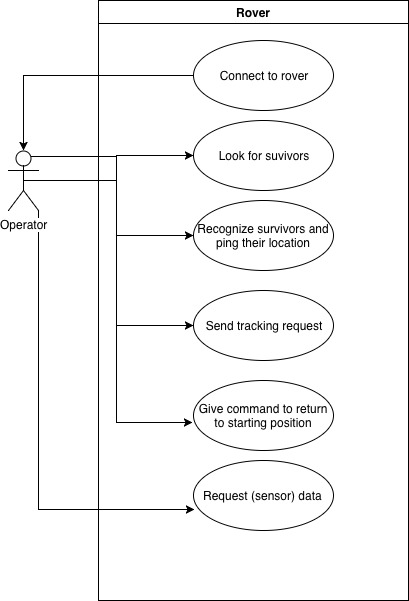
\includegraphics[width=\linewidth]{UseCaseDiagram.jpeg}
 	\subsection{Domain model}
 	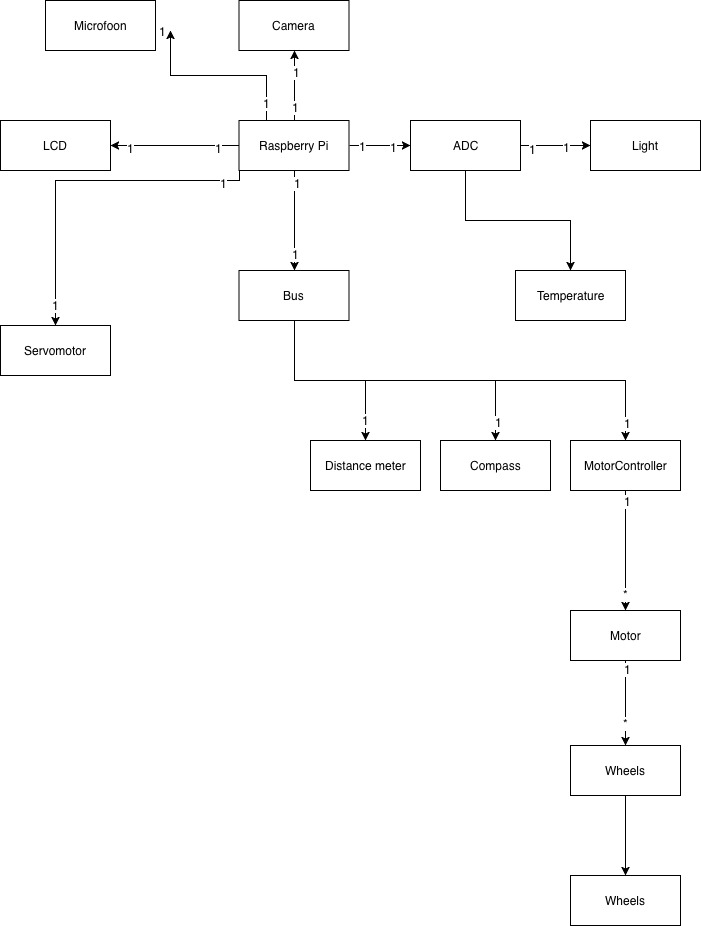
\includegraphics[width=\linewidth]{DomainModel.jpeg}
 	\newpage
 	\section{Testing}
 	In the fourth sprint we conducted multiple tests:
 	\subsection{General tests}
 	\begin{table}[H]
 		\centering
 		\begin{tabularx}{\linewidth}{|X|X|}
 			\hline
 			\textbf{ID} &1\\
 			\hline
 			\textbf{Testgoal} &Proof that it can be remote-controlled successfully via the camera\\
 			\hline
 			\textbf{Version} &1\\
 			\hline
 			\textbf{Testers} &Mustafa, Yoshio\\
 			\hline
 			\textbf{Date} &21 Dec 2018 at 2:30pm\\
 			\hline
 			\textbf{Location} &AUAS, WBH3\\
 			\hline
 			\textbf{Device(s)} &MacOS, Chrome\\
 			\hline
 			\textbf{Approach} &Operator cannot see rover. He/she can only see the web interface. 	Therefore, the camera on the rover must only be used to control.\\
 			\hline
 			\textbf{Proof} &Video demonstration\\
 			\hline
 			\textbf{Conclusion} &Test successful. Operator is able to control the rover using only the camera on the rover.\\
 			\hline
 		\end{tabularx}
 		\caption{Testcase 1}
 		\label{table:Testcase 1}   
 	\end{table}
	 \begin{table}[H]
	 	\centering
	 	\begin{tabularx}{\linewidth}{|X|X|}
	 		\hline
	 		\textbf{ID} &2\\
	 		\hline
	 		\textbf{Testgoal} &Proof that it can recognize faces\\
	 		\hline
	 		\textbf{Version} &1\\
	 		\hline
	 		\textbf{Testers} &Mustafa, Yoshio\\
	 		\hline
	 		\textbf{Date} &21 Dec 2018 at 1pm\\
	 		\hline
	 		\textbf{Location} &AUAS, WBH3\\
	 		\hline
	 		\textbf{Device(s)} &MacOS, Chrome\\
	 		\hline
	 		\textbf{Approach} &Mr Bean's face is trained and is the only face trained. We first show Mr Bean's face. His face should be recognized. Afterwards we show another person's face. That person's face should be unknown and most certainly not to be recognized as Mr Bean.\\
	 		\hline
	 		\textbf{Proof} &Video demonstration\\
	 		\hline
	 		\textbf{Conclusion} &The test was successful. Mr Bean's face was recognized at a percentage of 50\%. Our own was considered to be unknown. There is, however, a significant delay of ~1.5 seconds relative to real-time.\\
	 		\hline
	 	\end{tabularx}
	 	\caption{Testcase 2}
	 	\label{table:Testcase 2}   
	 \end{table}
 	\begin{table}[H]
 		\centering
 		\begin{tabularx}{\linewidth}{|X|X|}
 			\hline
 			\textbf{ID} &3\\
 			\hline
 			\textbf{Testgoal} &Proof that light turns on when it's dark\\
 			\hline
 			\textbf{Version} &1\\
 			\hline
 			\textbf{Testers} &Yoshio\\
 			\hline
 			\textbf{Date} &21 Dec 2018 at 3:30pm\\
 			\hline
 			\textbf{Location} &AUAS, WBH3\\
 			\hline
 			\textbf{Device(s)} &Windows 10, Chrome\\
 			\hline
 			\textbf{Approach} &Cover the rover with something like a blanket. The light should then turn on. Removing the blanket should result in the light turning off.\\
 			\hline
 			\textbf{Proof} &Video demonstration\\
 			\hline
 			\textbf{Conclusion} &Test successful. Covering causes the light to turn on, removing cover turns it off.\\
 			\hline
 		\end{tabularx}
 		\caption{Testcase 3}
 		\label{table:Testcase 3}   
 	\end{table}
 	\begin{table}[H]
 	\centering
	 	\begin{tabularx}{\linewidth}{|X|X|}
	 		\hline
	 		\textbf{ID} &4\\
	 		\hline
	 		\textbf{Testgoal} &Proof that light turns on when it's dark\\
	 		\hline
	 		\textbf{Version} &1\\
	 		\hline
	 		\textbf{Testers} &Mustafa, Yoshio\\
	 		\hline
	 		\textbf{Date} &21 Dec 2018 at 2pm\\
	 		\hline
	 		\textbf{Location} &AUAS, WBH3\\
	 		\hline
	 		\textbf{Device(s)} &MacOS, Chrome\\
	 		\hline
	 		\textbf{Approach} &Type text into text field on the web interface. Subsequently check if text can be seen on the display.\\
	 		\hline
	 		\textbf{Proof} &Video demonstration\\
	 		\hline
	 		\textbf{Conclusion} &Test was successful. We followed the instructions, no problems arose.\\
	 		\hline
	 	\end{tabularx}
 	\caption{Testcase 4}
 	\label{table:Testcase 4}   
	\end{table}
	\begin{table}[H]
		\centering
		\begin{tabularx}{\linewidth}{|X|X|}
			\hline
			\textbf{ID} &5\\
			\hline
			\textbf{Testgoal} &Proof that temperature works\\
			\hline
			\textbf{Version} &1\\
			\hline
			\textbf{Testers} &Mustafa, Yoshio\\
			\hline
			\textbf{Date} &21 Dec 2018 at 3pm\\
			\hline
			\textbf{Location} &AUAS, WBH3\\
			\hline
			\textbf{Device(s)} &MacOS, Chrome\\
			\hline
			\textbf{Approach} &Put finger on sensor. The web interface should display a higher temperature (finger temperature > room temperature). Also use a cold drink and push against the sensor, this should decrease the temperature.\\
			\hline
			\textbf{Proof} &Video demonstration\\
			\hline
			\textbf{Conclusion} &Test unsuccessful. Probably calculation mistake. The temperature decreases when temperature is higher and decreases when lower.\\
			\hline
		\end{tabularx}
		\caption{Testcase 5}
		\label{table:Testcase 5}   
	\end{table}
	\begin{table}[H]
		\centering
		\begin{tabularx}{\linewidth}{|X|X|}
			\hline
			\textbf{ID} &6\\
			\hline
			\textbf{Testgoal} &Proof that distance sensor works\\
			\hline
			\textbf{Version} &1\\
			\hline
			\textbf{Testers} &Mustafa, Yoshio\\
			\hline
			\textbf{Date} &21 Dec 2018 at 2pm\\
			\hline
			\textbf{Location} &AUAS, WBH3\\
			\hline
			\textbf{Device(s)} &MacOS, Chrome\\
			\hline
			\textbf{Approach} &Put hand in front of sensor and move forward/backwards. It should be able to accurately determine the distance of objects between itself when the distance is between 25cm and 55cm. It should also remain constant when the object doesn't move.\\
			\hline
			\textbf{Proof} &Video demonstration\\
			\hline
			\textbf{Conclusion} &Test successful. Moving hand closer than 25cm gives inaccurate measurements and the same goes for distances larger than 55cm. In between the distance is accurately measured and constant.\\
			\hline
		\end{tabularx}
		\caption{Testcase 6}
		\label{table:Testcase 6}   
	\end{table}
	\begin{table}[H]
		\centering
		\begin{tabularx}{\linewidth}{|X|X|}
			\hline
			\textbf{ID} &7\\
			\hline
			\textbf{Testgoal} &Proof that compass works\\
			\hline
			\textbf{Version} &1\\
			\hline
			\textbf{Testers} &Mustafa, Yoshio\\
			\hline
			\textbf{Date} &21 Dec 2018 at 2pm\\
			\hline
			\textbf{Location} &AUAS, WBH3\\
			\hline
			\textbf{Device(s)} &MacOS, Chrome\\
			\hline
			\textbf{Approach} &Turn rover 90 degrees. This should match a turn of a phone turning the same angle.\\
			\hline
			\textbf{Proof} &Video demonstration\\
			\hline
			\textbf{Conclusion} &Test unsuccessful. Probably a hardware/interference problem, because code seems to work for others.\\
			\hline
		\end{tabularx}
		\caption{Testcase 7}
		\label{table:Testcase 7}   
	\end{table}
	\begin{table}[H]
		\centering
		\begin{tabularx}{\linewidth}{|X|X|}
			\hline
			\textbf{ID} &8\\
			\hline
			\textbf{Testgoal} &Proof that backtracking works\\
			\hline
			\textbf{Version} &1\\
			\hline
			\textbf{Testers} &Mustafa, Yoshio\\
			\hline
			\textbf{Date} &21 Dec 2018 at 3pm\\
			\hline
			\textbf{Location} &AUAS, WBH3\\
			\hline
			\textbf{Device(s)} &MacOS, Chrome\\
			\hline
			\textbf{Approach} &Drive forward, then a 90 degree angle to either left/right. Drive forward. Then backtrack. It should return to its initial position.\\
			\hline
			\textbf{Proof} &Video demonstration\\
			\hline
			\textbf{Conclusion} &Test was unsuccessful due to one or more wheels not working fully. Also only driving forward and then backtracking, causes it to go more backwards then forwards. No attention has been given to the fact that the motors are running at full power until the last millisecond.\\
			\hline
		\end{tabularx}
		\caption{Testcase 8}
		\label{table:Testcase 8}   
	\end{table}
	\begin{table}[H]
		\centering
		\begin{tabularx}{\linewidth}{|X|X|}
			\hline
			\textbf{ID} &9\\
			\hline
			\textbf{Testgoal} &Proof that map corresponds to route taken\\
			\hline
			\textbf{Version} &1\\
			\hline
			\textbf{Testers} &Mustafa, Yoshio\\
			\hline
			\textbf{Date} &21 Dec 2018 at 3pm\\
			\hline
			\textbf{Location} &AUAS, WBH3\\
			\hline
			\textbf{Device(s)} &MacOS, Chrome\\
			\hline
			\textbf{Approach} &Drive forwards, then the operator should see that the line has moved forward. Drive an other direction then the operator should see that the line has moved into that direction.\\
			\hline
			\textbf{Proof} &Video demonstration\\
			\hline
			\textbf{Conclusion} &Line doesn't completely correspond to route taken due to the way the robot senses turns. The line is being generated though when it moves, but just not entirely accurate. Other approaches unfortunately weren't possible due to inconsistencies as well. Therefore, this is as of now the best we can do.\\
			\hline
		\end{tabularx}
		\caption{Testcase 9}
		\label{table:Testcase 9}   
	\end{table}
	\begin{table}[H]
		\centering
		\begin{tabularx}{\linewidth}{|X|X|}
			\hline
			\textbf{ID} &10\\
			\hline
			\textbf{Testgoal} &Proof that when backtracking the rover stops moving when an object is behind it (25-55cm)\\
			\hline
			\textbf{Version} &1\\
			\hline
			\textbf{Testers} &Yoshio\\
			\hline
			\textbf{Date} &21 Dec 2018 at 4pm\\
			\hline
			\textbf{Location} &AUAS, WBH3\\
			\hline
			\textbf{Device(s)} &Windows 10, Chrome\\
			\hline
			\textbf{Approach} &Drive forward, then place an object behind it 25-55cm. Then activate backtrack. It should stop almost immediately.\\
			\hline
			\textbf{Proof} &Video demonstration\\
			\hline
			\textbf{Conclusion} &Test successful. It does, however, tend to drive a little too much backwards.\\
			\hline
		\end{tabularx}
		\caption{Testcase 10}
		\label{table:Testcase 10}   
	\end{table}
	\begin{table}[H]
		\centering
		\begin{tabularx}{\linewidth}{|X|X|}
			\hline
			\textbf{ID} &11\\
			\hline
			\textbf{Testgoal} &Proof that when backtracking the rover moves the distance sensor via the servo so it can detect objects from different angles as well.\\
			\hline
			\textbf{Version} &1\\
			\hline
			\textbf{Testers} &Yoshio\\
			\hline
			\textbf{Date} &21 Dec 2018 at 3:45pm\\
			\hline
			\textbf{Location} &AUAS, WBH3\\
			\hline
			\textbf{Device(s)} &Windows 10, Chrome\\
			\hline
			\textbf{Approach} &Drive forward, then place an object behind it 25-55cm within a degree of 90. Then activate backtrack. It should stop almost immediately.\\
			\hline
			\textbf{Proof} &None\\
			\hline
			\textbf{Conclusion} &Test successful when little interference is present.\\
			\hline
		\end{tabularx}
		\caption{Testcase 11}
		\label{table:Testcase 11}   
	\end{table}
	\subsection{Acceptance tests}
	\begin{table}[H]
		\centering
		\begin{tabularx}{\linewidth}{|X|X|}
			\hline
			\textbf{ID} &1\\
			\hline
			\textbf{Name} &Connect with rover\\
			\hline
			\textbf{Basis} &\begin{itemize}
								\item Use case: connect with rover
								\item User story: connect app to rover
							\end{itemize}\\
			\hline
			\textbf{Figure(s)} &1, 2 \\
			\hline
			\textbf{Pre-conditions} & \begin{itemize}
									  	\item Rover nearby
									  	\item Mobile app opened
									  	\item Connected through Wifi with rover hotspot
									  \end{itemize}\\
			\hline
			\textbf{Test} &Given: List of rovers to connect to\\
						&When: Select rover from list\\
						&Then: Selected and visual cue that rover is selected\\
						&\\
						&Given: List of rovers to connect to while rover already selected\\
						&When: Select other rover from list\\
						&Then: Selected and visual cue that other rover is selected\\
						&\\
						&Given: List of rovers to connect to while rover already selected\\
						&When: Select same rover from list\\
						&Then: Selection and visual cue remain the same\\
						&\\
						&Given: Selected rover from list\\
						&When: Click on connect button\\
						&Then: See Rover UI with rover no. of selected rover\\
			\hline
			\textbf{Remarks} &When I try to go through the list, the item I put my finger upon is automatically selected as well, even when my intention wasn't to.\\
			\hline
		\end{tabularx}
		\caption{Acceptance test 1}
		\label{table:Acceptance test 1}   
	\end{table}
	\begin{table}[H]
		\centering
		\begin{tabularx}{\linewidth}{|X|X|}
			\hline
			\textbf{ID} &2\\
			\hline
			\textbf{Name} &See what rover sees\\
			\hline
			\textbf{Basis} &\begin{itemize}
				\item Use case: look for survivors on flat surfaces
				\item User story: see what rover sees
			\end{itemize}\\
			\hline
			\textbf{Figure(s)} &1, 2 \\
			\hline
			\textbf{Pre-conditions} & \begin{itemize}
				\item Connected with rover
			\end{itemize}\\
			\hline
			\textbf{Test} &Given: Rover UI of a rover\\
			&Then: See what camera of rover sees through UI\\
			&\\
			&Given: Rover UI of a rover\\
			&Then: See what rover number\\
			&\\	
			&Given: Rover UI of a rover\\
			&Then: See rover IP and port\\
			\hline
			\textbf{Remarks} &When I go to a dummy UI which has obviously no camera feed, then I get this ugly 404 error.\\
			\hline
		\end{tabularx}
		\caption{Acceptance test 2}
		\label{table:Acceptance test 2}   
	\end{table}
	\subsection{Use-case testing}
		\begin{table}[H]
		\centering
		\begin{tabularx}{\linewidth}{|X|X|}
			\hline
			\textbf{Use-case id} &1\\
			\hline
			\textbf{Use-case name} &Tracking the location of the rover.\\
			\hline
			\textbf{Primary actor} &Rover operator\\
			\hline
			\textbf{Secondary actor} &Rover\\
			\hline
			\textbf{Pre-conditions} &\begin{itemize}
										\item Rover operator has established a connection between the web interface and the rover.
										\item Rover operator has controller.
									\end{itemize}\\
			\hline
			\textbf{Success guarantee} &Rover operator tracks the location of the rover through a map on the web interface\\
			\hline
			\textbf{Main success scenario} &\begin{itemize}
												\item Rover operator uses controller to drive either forward, backward, left, or right.
												\item Rover operator sees location of the rover changing in the same direction as he/she is moving it.
											\end{itemize}\\
			\hline
			\textbf{Exceptions} &-\\
			\hline
			\textbf{Special requirements} &When the rover is unable to move in a certain direction because of an obstacle then this should be reflected in the map as not having moved.\\
			\hline
		\end{tabularx}
		\caption{Use-case test 1}
		\label{table:Use-case test 1}   
	\end{table}
	\begin{table}[H]
		\centering
		\begin{tabularx}{\linewidth}{|X|X|}
			\hline
			\textbf{Use-case id} &2\\
			\hline
			\textbf{Use-case name} &Backtracking the rover.\\
			\hline
			\textbf{Primary actor} &Rover operator\\
			\hline
			\textbf{Secondary actor} &Rover\\
			\hline
			\textbf{Pre-conditions} &\begin{itemize}
				\item Rover operator has established a connection between the web interface and the rover.
				\item Rover operator has controller
			\end{itemize}\\
			\hline
			\textbf{Success guarantee} &Rover returns to initial position in the opposite way as it has moved to its current position.\\
			\hline
			\textbf{Main success scenario} &\begin{itemize}
				\item Rover operator uses controller to drive either forward, backward, left, or right.
				\item Rover operator turns backtracking on.
				\item Rover goes back to its initial position.
			\end{itemize}\\
			\hline
			\textbf{Exceptions} &-\\
			\hline
			\textbf{Special requirements} &Moments where the rover stopped are ignored. So, the rover drives back directly without stopping.\\
			\hline
		\end{tabularx}
		\caption{Use-case test 2}
		\label{table:Use-case test 2}   
	\end{table}
	\begin{table}[H]
	\centering
	\begin{tabularx}{\linewidth}{|X|X|}
		\hline
		\textbf{Use-case id} &3\\
		\hline
		\textbf{Use-case name} &See data about rover\\
		\hline
		\textbf{Primary actor} &Rover operator\\
		\hline
		\textbf{Secondary actor} &Rover\\
		\hline
		\textbf{Pre-conditions} &\begin{itemize}
			\item Rover operator is on the control page/view.
		\end{itemize}\\
		\hline
		\textbf{Success guarantee} &Rover operator can read the following in the interface:
		\begin{itemize}
			\item Temperature at rover
			\item Camera shown at rover
			\item Position of servo of rover
			\item Distance between rover and object in front of it
			\item IP of rover
			\item Port at which  the operator is connected to
			\item Rover number	
		\end{itemize}
		\\
		\hline
		\textbf{Main success scenario} &\begin{enumerate}
			\item Rover operator reads temperature of from interface.
			\item Rover operator reads what camera of rover he/she sees in the interface.
			\item Rover operator reads position of servo.
			\item Rover operator reads IP of rover.
			\item Rover operator reads what port he/she is connected to.
			\item Rover operator reads which rover this is.	
		\end{enumerate}\\
		\hline
		\textbf{Exceptions} &-\\
		\hline
		\textbf{Special requirements} &-\\
		\hline
		\end{tabularx}
		\caption{Use-case test 3}
		\label{table:Use-case test 3}   
	\end{table}
 	\section{Design model}
 	As with the analysis of our product the design model contains multiple elements. These elements are as follows:
 	\begin{itemize}
 		\item Class diagram
 		\item Sequence diagram
 		\item Communication diagram
 		\item Hardware architecture
 	\end{itemize}
 	The design model answers the question of "how, in detail, is the product built?"
 	\subsection{Class diagram}
 		\begin{figure}[H]
 		\centering
 		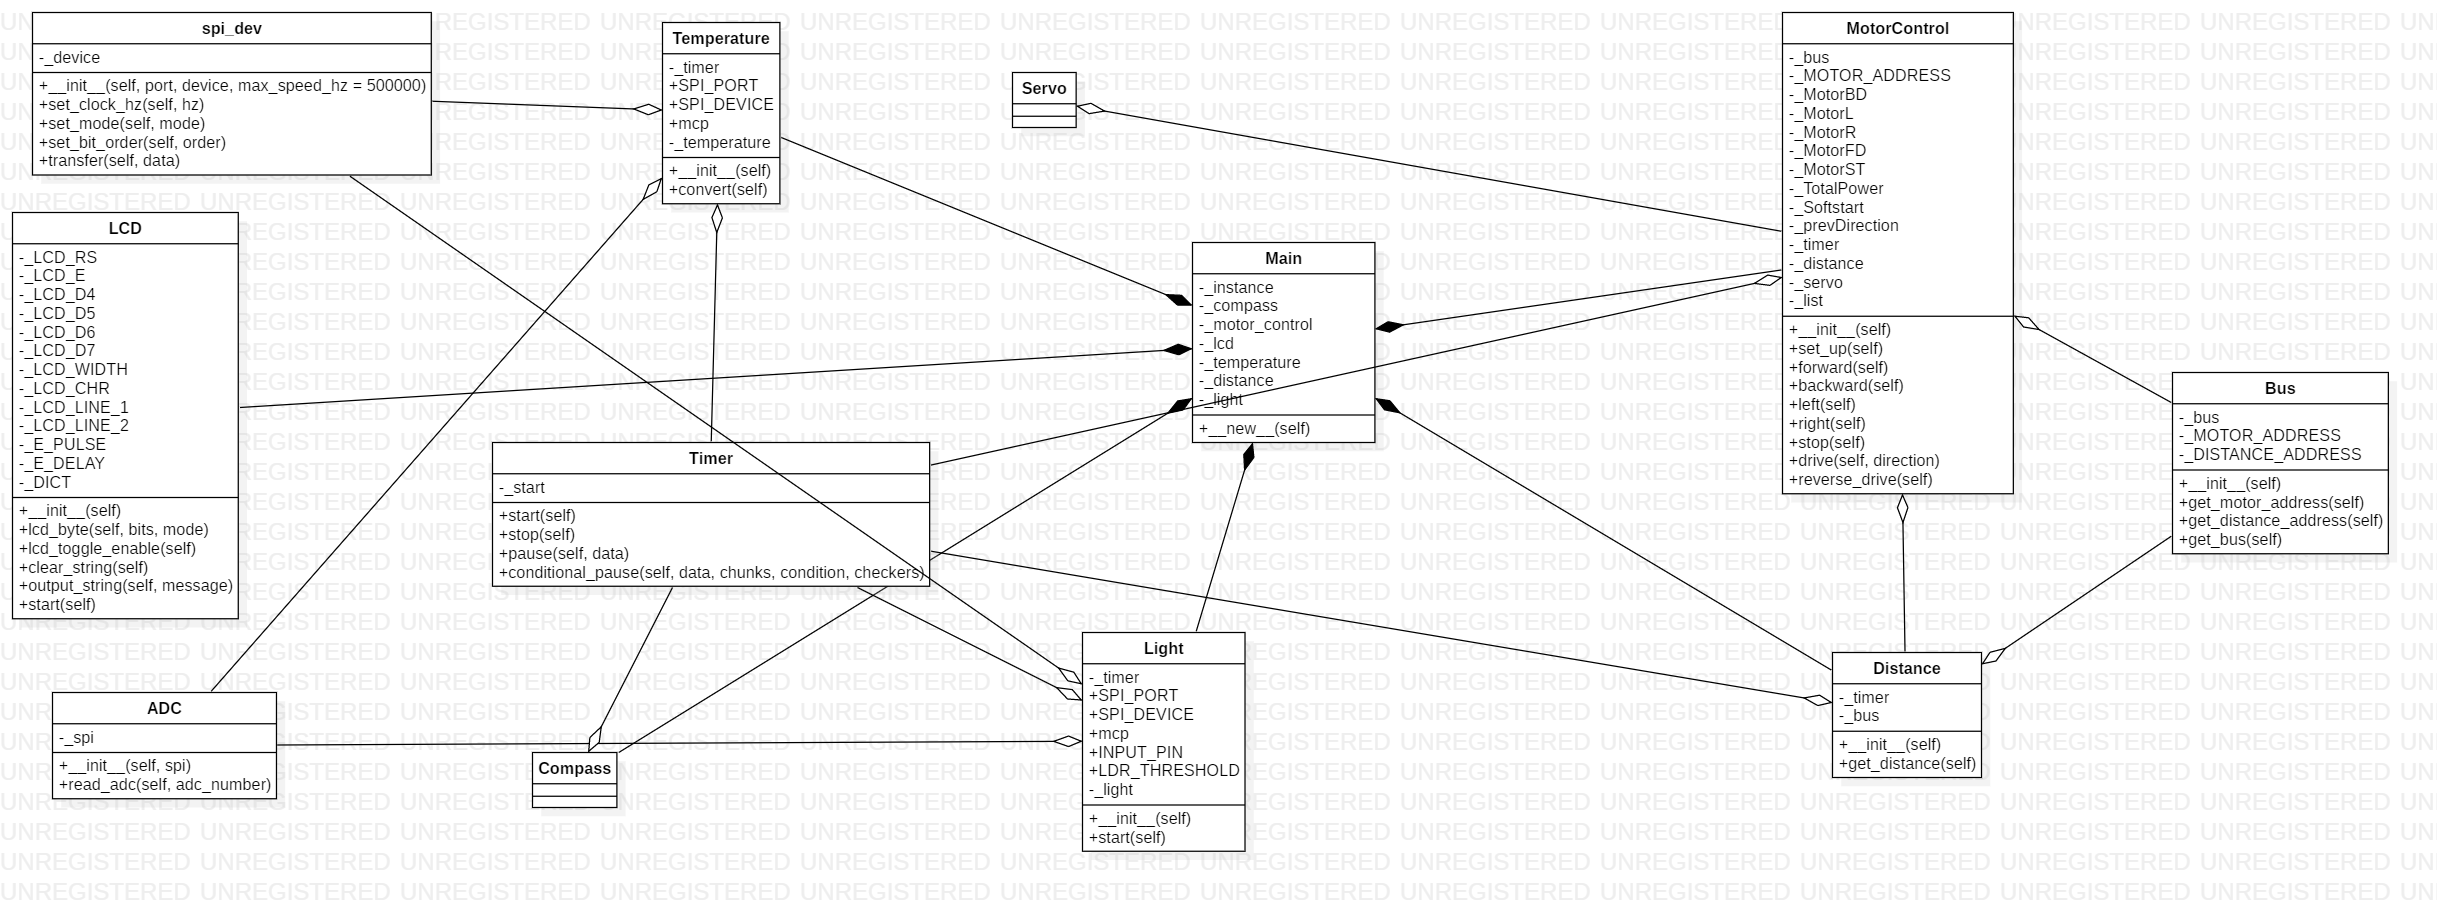
\includegraphics[width=\linewidth]{MobileClassDiagram.png}\\
 		\caption{Class diagram for the mobile application}
 		\end{figure}
 	\subsection{Sequence diagram}
 	\subsection{Communication diagram}
 	\begin{figure}[H]
 		\centering
 		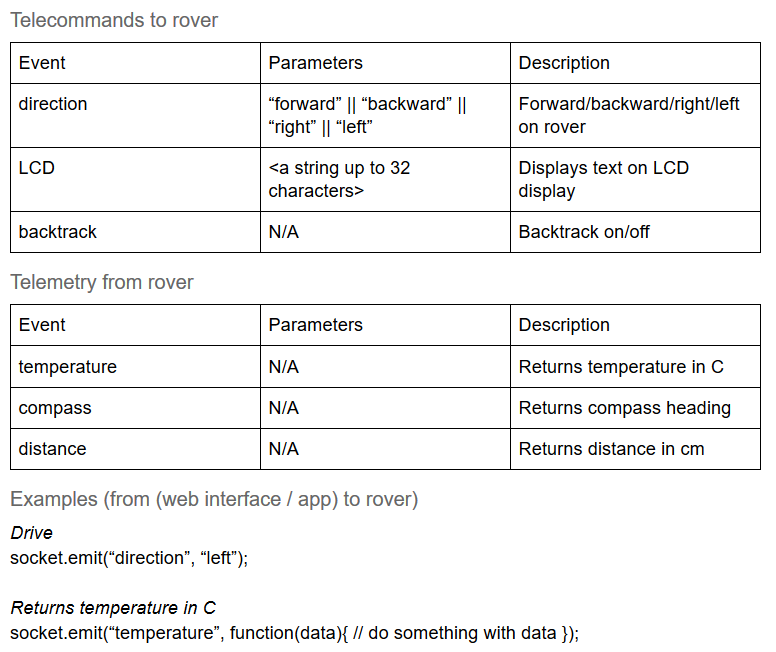
\includegraphics[width=\linewidth]{ComDiagram.png}\\
 		\caption{Diagram of the communication of our product}
 	\end{figure}
 	\subsection{Hardware architecture}
 	\begin{figure}[H]
 		\centering
 		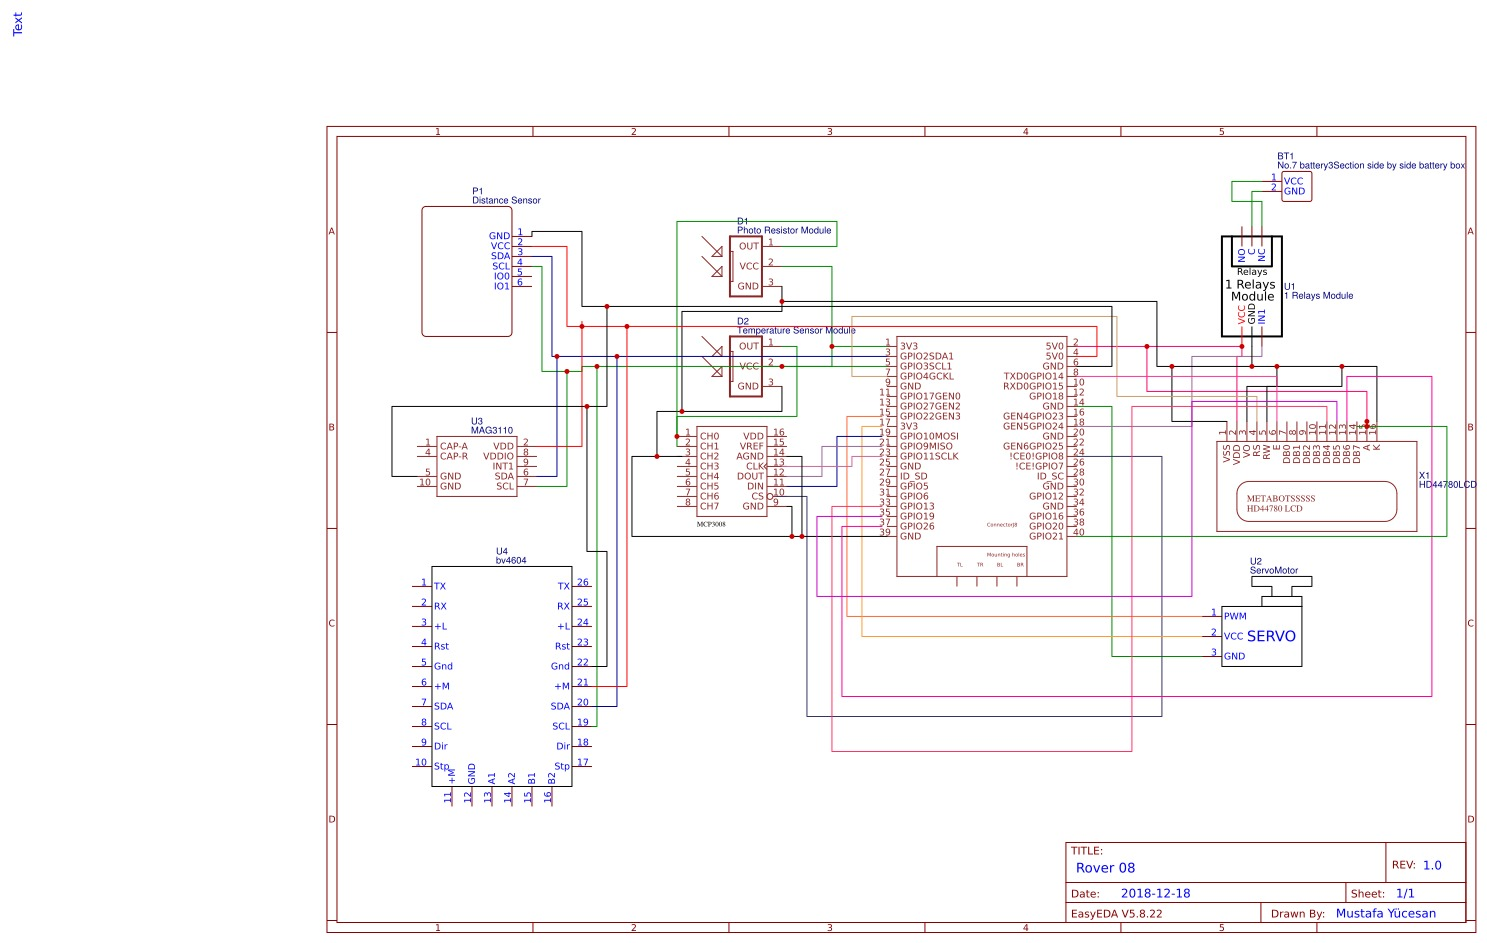
\includegraphics[width=\linewidth]{HardwareArch.jpeg}\\
 		\caption{Diagram of our product's architecture}
 	\end{figure}
 	\section{Installation manual}
 	\section{User manual}
\end{document}	